%--------------------------------------------%
% Template Beamer para Apresentações da UFRN %
% by alcemygvseverino@gmail.com              %
% Baseado em MIT Beamer Template			 %
% versao 1.1								 %
% Atualizado em 14/05/2016					 %
%--------------------------------------------%
\documentclass[t,9pt,aspectratio=169]{beamer}
% Para alterar a linguagem do documento
\usepackage[utf8]{inputenc}
% Para seguir as normas da ABNT de citacao e referencias
\usepackage[alf]{abntex2cite}
% Para incluir figuras
\usepackage{graphicx}
% Para melhor ajuste da posisao das figuras
\usepackage{float}
% Para ajustar as dimensoes do layout da pagina
\usepackage{geometry}
% Para formatar estrutura e informacoes de formulas matematicas
% Para incluir simbolos especiais em formulas matematicas
% Para incluir links nas referencias
%\usepackage{url}
% Para incluir paginas de documentos .pdf externos
\usepackage{pgfpages}
% Para ajustar o estilo dos contadores
\usepackage{enumerate}
%\usepackage{benstyle}
% Para modificar a cor do texto
\usepackage{color}
% Para incluir condicoes
\usepackage{ifthen}
\usepackage{amsmath,amssymb,amsthm} 
\everymath{\displaystyle}
\usepackage{dsfont}
\usepackage{caption}
\usepackage{physics}
\usepackage{tikz}
\usetikzlibrary{calc}
\usepackage{pgfplots}
\usepackage{pgfplotstable}
\usepackage{comment}
\pgfplotsset{compat=1.14}
\usetikzlibrary{decorations.pathmorphing}
\usepackage{cancel}
\captionsetup{
  format=plain,
  margin=10 mm,
}

% Para colocar legendas em algo que nao e float
\usepackage{capt-of}

\mode<presentation>{
	% Para definir o tema do slide
	\usetheme{Berlin}
	% Para difinir cores e background
	\usecolortheme{ufrn}
	% Para numerar as figuras
	\setbeamertemplate{caption}[numbered]

	\setbeamertemplate{navigation symbols}{}

}
%%%% Various Characters %%%
\def\Re{\mathrm{Re}\,}
\def\Im{\mathrm{Im}\,}
\def\D{\,\mathrm{d}}
\def\I{\mathrm{i}}
\def\E{\mathrm{e}}
\def\bcE{\bm{\cE}}
\newcommand*{\rth}{\mathrm{th}}
\def\imath{\mathrm{i}}
%%% Sebastian definitions %%%
\def\bP{\bm{P}}
\def\beps{\bm{\varepsilon}}
\def\bepsr{\beps_{\bm{\rho}}}
\def\brho{\bm{\rho}}
\def\hf{\hat{\bm{f}}}
\def\LHC{\Lambda_{s}^{\rm{HC}}}
\def\bnu{\bm{\nu}}
\def\bmu{\bm{\mu}}
\def\bA{\bm{A}}
\def\hu{\hat{\u}}
\def\hv{\hat{\v}}
\def\hy{\hat{\y}}
\def\hx{\hat{\x}}
\def\e{\bm{e}}
\def\hxi{\hat{\bxi}}
\def\bxi{\bm{\xi}}
\def\f{\bm{f}}
\def\b{\bm{b}}
\def\bc{\bm{c}}
\def\hbc{\hat{\bc}}
\def\x{\bm{x}}
\def\y{\bm{y}}
\def\0{\bm{0}}
\def\v{\bm{v}}
\def\u{\bm{u}}
\def\z{\bm{z}}
\def\p{\bm{p}}
\def\hatt{\hat{\t}}
\def\w{\bm{w}}
\def\sh{\s_h}
\def\vh{\bm{v}_h}
\def\uh{\bm{u}_h}
\def\zh{\bm{z}_h}
\def\wh{\bm{w}_h}
\def\q{\bm{q}}

\def\zn{\mathbf{z}^{(n)}}
\def\xn{\mathbf{x}^{(n)}}

\def\un{\mathbf{u}^{(n)}}
\def\vn{\mathbf{v}^{(n)}}
\newcommand*{\inp}[2]{\langle #1, #2 \rangle}
\def\cVN{\cV^{N}}
\def\cVm{\cV^{m}}
\def\cVM{\cV^{m}}
%%% Sebastian commands %%%
\newcommand\qan{{\quad\hbox{and}\quad}}
\newcommand\disp{\displaystyle}
%\newcommand{\norm}[1]{{||#1||}}
%\newcommand{\wnormV}[1]{{||#1||_{\cV,1,\omega}}}
%\newcommand{\normdV}[1]{{||#1||_{\cV,2}}}



%%% Colours %%%
%\usepackage[dvipsnames]{xcolor}
\newcommand*{\BLUE}[1]{{\color{blue}#1}}
\newcommand*{\RED}[1]{{\color{red}#1}}
\newcommand*{\GREEN}[1]{{\color{green}#1}}
\newcommand*{\CY}[1]{{\color{cyan}#1}}
\newcommand*{\MG}[1]{{\color{magenta}#1}}
\DefineNamedColor{named}{Purple}{cmyk}{0.45,0.86,0,0}
\newcommand*{\PURP}[1]{{\color[named]{Purple}#1}}
\DefineNamedColor{named}{JungleGreen} {cmyk}{0.99,0,0.52,0}
\newcommand*{\GR}[1]{{\color[named]{JungleGreen}#1}}
\DefineNamedColor{named}{orange} {rgb}{1,0.55,0}
\newcommand*{\ORNG}[1]{{\color[named]{orange}#1}}
\DefineNamedColor{named}{applegreen}{rgb}{0.55, 0.71, 0.0}
\usepackage[normalem]{ulem}
\newcommand*{\MGS}[1]{{\color{magenta}\sout{#1}}}
\newcommand*{\RDS}[1]{{\color{red}\sout{#1}}}
\newcommand*{\CYS}[1]{{\color{cyan}\sout{#1}}}
\newcommand*{\PS}[1]{{\color[named]{Purple}\sout{#1}}}

%%% Script letters %%%
\newcommand*{\cA}{\mathcal{A}} 
\newcommand*{\cB}{\mathcal{B}}
\newcommand*{\cC}{\mathcal{C}}
\newcommand*{\cD}{\mathcal{D}}
\newcommand*{\cE}{\mathcal{E}}
\newcommand*{\cF}{\mathcal{F}}
\newcommand*{\cG}{\mathcal{G}}
\newcommand*{\cH}{\mathcal{H}}
\newcommand*{\cI}{\mathcal{I}}
\newcommand*{\cJ}{\mathcal{J}}
\newcommand*{\cK}{\mathcal{K}}
\newcommand*{\cL}{\mathcal{L}}
\newcommand*{\cM}{\mathcal{M}}
\newcommand*{\cN}{\mathcal{N}}
\newcommand*{\cQ}{\mathcal{Q}}
\newcommand*{\cR}{\mathcal{R}}
\newcommand*{\cO}{\mathcal{O}}
\newcommand*{\cP}{\mathcal{P}}
\newcommand*{\cS}{\mathcal{S}}
\newcommand*{\cU}{\mathcal{U}}
\newcommand*{\cT}{\mathcal{T}}
\newcommand*{\cV}{\mathcal{V}}
\newcommand*{\cW}{\mathcal{W}}
\newcommand*{\cX}{\mathcal{X}}
\newcommand*{\cY}{\mathcal{Y}}
\newcommand*{\cZ}{\mathcal{Z}}

%%% Bold face letters %%%
\newcommand*{\bbA}{\mathbb{A}} 
\newcommand*{\bbB}{\mathbb{B}}
\newcommand*{\bbC}{\mathbb{C}}
\newcommand*{\bbD}{\mathbb{D}}
\newcommand*{\bbE}{\mathbb{E}}
\newcommand*{\bbF}{\mathbb{F}}
\newcommand*{\bbG}{\mathbb{G}}
\newcommand*{\bbH}{\mathbb{H}}
\newcommand*{\bbI}{\mathbb{I}}
\newcommand*{\bbJ}{\mathbb{J}}
\newcommand*{\bbK}{\mathbb{K}}
\newcommand*{\bbL}{\mathbb{L}}
\newcommand*{\bbM}{\mathbb{M}}
\newcommand*{\bbN}{\mathbb{N}}
\newcommand*{\bbQ}{\mathbb{Q}}
\newcommand*{\bbR}{\mathbb{R}}
\newcommand*{\bbO}{\mathbb{O}}
\newcommand*{\bbP}{\mathbb{P}}
\newcommand*{\bbS}{\mathbb{S}}
\newcommand*{\bbU}{\mathbb{U}}
\newcommand*{\bbT}{\mathbb{T}}
\newcommand*{\bbV}{\mathbb{V}}
\newcommand*{\bbW}{\mathbb{W}}
\newcommand*{\bbX}{\mathbb{X}}
\newcommand*{\bbY}{\mathbb{Y}}
\newcommand*{\bbZ}{\mathbb{Z}}

%%% Roman letters %%%
\newcommand*{\rA}{\mathrm{A}} 
\newcommand*{\rB}{\mathrm{B}}
\newcommand*{\rC}{\mathrm{C}}
\newcommand*{\rD}{\mathrm{D}}
\newcommand*{\rE}{\mathrm{E}}
\newcommand*{\rF}{\mathrm{F}}
\newcommand*{\rG}{\mathrm{G}}
\newcommand*{\rH}{\mathrm{H}}
\newcommand*{\rI}{\mathrm{I}}
\newcommand*{\rJ}{\mathrm{J}}
\newcommand*{\rK}{\mathrm{K}}
\newcommand*{\rL}{\mathrm{L}}
\newcommand*{\rM}{\mathrm{M}}
\newcommand*{\rN}{\mathrm{N}}
\newcommand*{\rQ}{\mathrm{Q}}
\newcommand*{\rR}{\mathrm{R}}
\newcommand*{\rO}{\mathrm{O}}
\newcommand*{\rP}{\mathrm{P}}
\newcommand*{\rS}{\mathrm{S}}
\newcommand*{\rU}{\mathrm{U}}
\newcommand*{\rT}{\mathrm{T}}
\newcommand*{\rV}{\mathrm{V}}
\newcommand*{\rW}{\mathrm{W}}
\newcommand*{\rX}{\mathrm{X}}
\newcommand*{\rY}{\mathrm{Y}}
\newcommand*{\rZ}{\mathrm{Z}}
\newcommand{\myred}[1]{{\color{red}#1}}
\newcommand{\myyellow}[1]{{\color{nyellow}#1}}
\newcommand{\myyell}[1]{{\color{ORNL_gray}#1}}
\newcommand{\mypink}[1]{{\color{taaluminium}#1}}
\newcommand{\mygreen}[1]{{\color{green}#1}}
\newcommand{\mydarkgreen}[1]{{\color{JungleGreen}#1}}
\newcommand{\mypurp}[1]{{\color{uuxpurple}#1}}
\newcommand{\myorg}[1]{{\color{taorange}#1}}
\newcommand{\myblue}[1]{{\color{blue}#1}}
\newcommand{\mygold}[1]{{\color{uu2terra}#1}}
\newcommand{\myblack}[1]{{\color{black}#1}}
\usepackage{bm}
\usepackage{color}
%--------------Cosas definidas por mi----------------------

%----------------------------------------------------------------------------------------
%	NEW COMMANDS
%---------------------------------------------------------------------------------------








% Título
 
\title[ Project by Theorymesh]{ Analysis of components of food production  for sustainability in Canada  }
% Data
\date{August 26, 2021 }
% Autores
\author[Team 10]{
	{  
\includegraphics[scale=0.3]{figures/theorymesh}   \\ Chris Bunio, Cuneyt Akcora.     }\\
	{\small S. Moraga \inst{1}  ,\,
	{\small  E. Pacheco \inst{2}},\,
            T. Pender   \inst{3},\, I. Vin\'icius  \inst{4} ,\, S. Yeal   \inst{5} \\  
           
\includegraphics[scale=0.08]{figures/seba}
           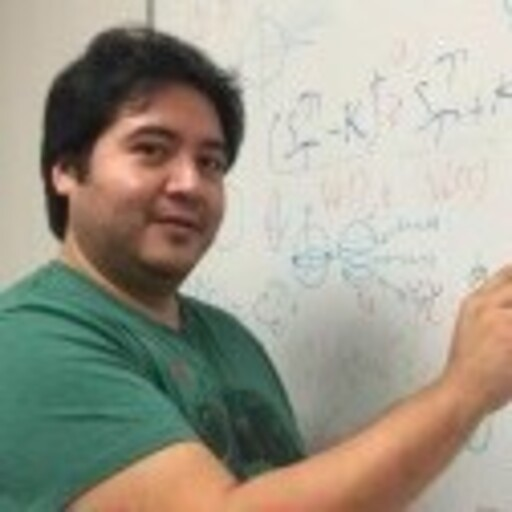
\includegraphics[scale=0.08]{figures/edgar}
           
\includegraphics[scale=0.08]{figures/tkn}
           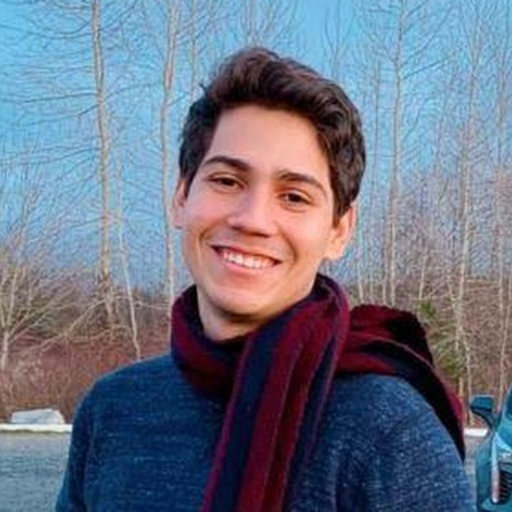
\includegraphics[scale=0.08]{figures/igor}
           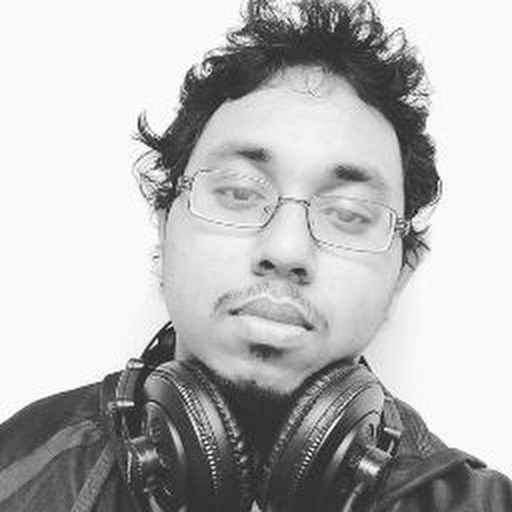
\includegraphics[scale=0.08]{figures/simon}
	 }  \\
}
    
% Instituto
\institute[Simon Fraser University]{

	\inst{1}%
	Department of Mathematics. Simon Fraser University. Canada. 
    \inst{2}%
	Department of Mathematics and Statistics, University of Calgary. \\
	    \inst{3}%
	Department of Mathematics and Computer Science, University of Lethbridge.
	    \inst{4}%
	Department of $\ldots$, University of $\ldots$.\\
	    \inst{5}%
	Department of $\ldots$, University of $\ldots$.\\}

\AtBeginSection[]
{
 \begin{frame}<beamer>
 
 \frametitle{Outline}
 \tableofcontents[currentsection]
 \end{frame}
}
    
% Logo do canto inferior direito
\pgfdeclareimage[height=0.7cm]{logo_UFRN}{figuras/sfu}
%\logo{
%	\vspace*{-0.25cm}
%   \pgfuseimage{logo_UFRN}
%	\hspace*{-0.05cm}}


\begin{document}
% Sumário
\frame{
\includegraphics[scale=0.3]{figures/pims-logo-25} \hspace{9cm} 
\includegraphics[scale=0.08]{figures/m2pilogo}  \titlepage}
 
%-------------------------------------------------------------------------------------------------------------------------
% Section: Introduction
%   - introduce problem
%   - why is the problem important
%-------------------------------------------------------------------------------------------------------------------------
\section{Introduction}
\begin{frame}{Motivation problem}
 \begin{block}{Goal}
Here ...
 \end{block}
 
 
 \vspace{-0.5cm}
\begin{center}
\begin{columns}
\column{0.08\paperwidth}
\begin{center}
    \vspace{0.3cm}
\myred{Input} \\
Data %\\
%$d$ finite, but \myred{large}
\end{center}

\column{0.03\paperwidth}

\vspace{0.7cm}
{\large \textbf{$\bm{\rightarrow}$}}

\column{0.12\paperwidth}
\begin{block}{}
\begin{center}
{\large \bf Blackbox model}
%{\Large Ex: PDEs, classification}
\end{center}
\end{block}


\column{0.03\paperwidth}

\vspace{0.7cm}
{\large \textbf{$\bm{\rightarrow}$}}

\column{0.13\paperwidth}
\begin{center}
    \vspace{0.1cm}
\mydarkgreen{Output} Information
\end{center}

\column{0.03\paperwidth}


 
\end{columns}
\end{center} \vfill
\end{frame}

%-------------------------------------------------------------------------------------------------------------------------
% Section: Interpretations and Results
%   - general trends in crop productivity; info given in way to appeal to a larger audience (Tom)
%   - Simon???????
%-------------------------------------------------------------------------------------------------------------------------

\section{Interpretations and Steps Forward}

\begin{frame}{Availability of information for producers}

\begin{center}
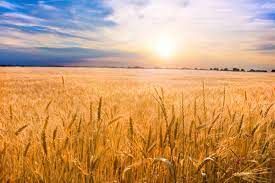
\includegraphics[width=10cm, height=1.75cm]{./figures/wheat.jpeg}
\end{center}

\begin{itemize}
 \item Information is power!
 \item Currently, the relavent information resides in technical journals that is penetrable only for researchers and experts in the field. 
 \item Needs to be available/intelligible to producers.
 \item The general sentiment conveyed by industry participants:
 \begin{itemize}
 \item There needs to be a change in the way that information is disseminated.
 \item It used to be that the when/where/how questions of crop production were passed by word of mouth: ``Do this because it has always worked.''
 \item This is no longer tenable with the rapidly changing climate/environmental conditions.
 \item Over the coming decades that will span a contemporary producer's career, they will invariably need to adjust their approaches.
 \end{itemize}
\end{itemize}

\end{frame}

\begin{frame}{What can be gleaned from the data?}
 
 \begin{center}
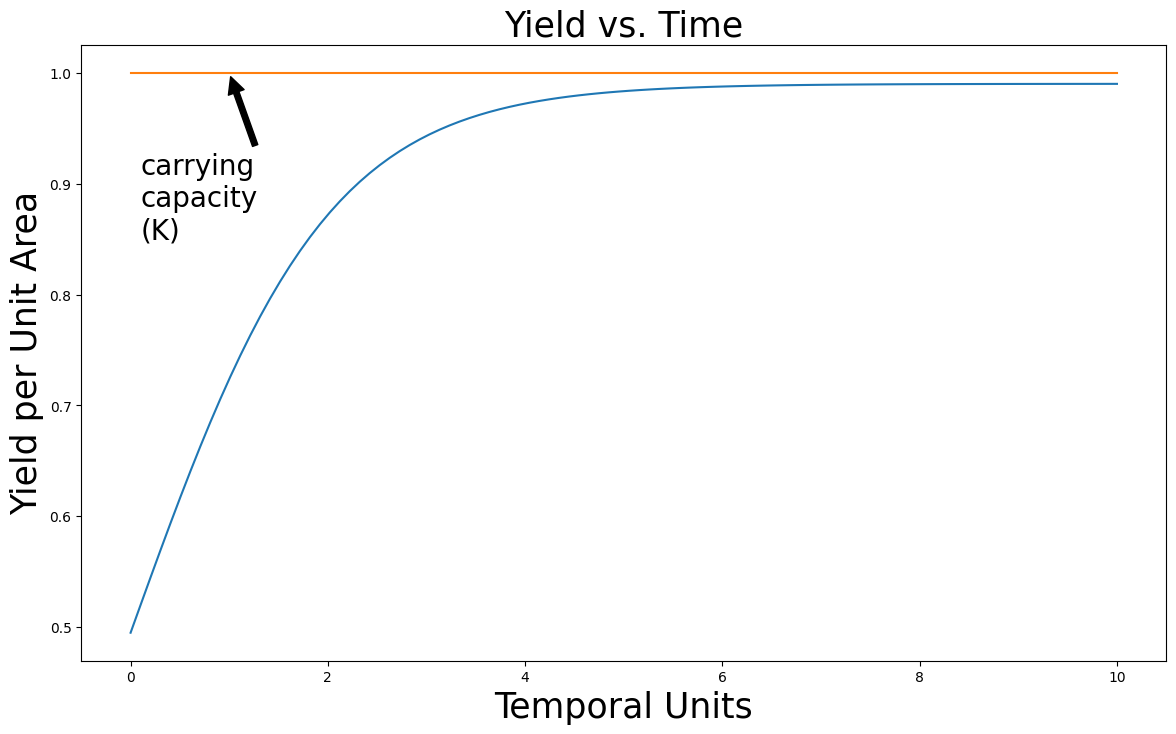
\includegraphics[scale=0.25]{./figures/yields.png}
 \end{center}
 
 \begin{itemize}
  \item $K = K(x_1, x_2, \dots, x_n)$, where no $x_i$ is a temporal variable.
 \end{itemize}
 
\end{frame}

\begin{frame}{Factors Affecting $K$}

\begin{center}

 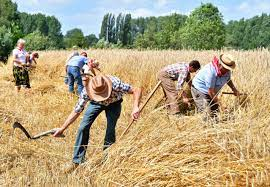
\includegraphics[width=3cm, height=2.75cm]{./figures/harvestOld}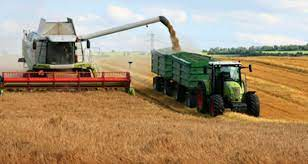
\includegraphics[width=3cm, height=2.75cm]{./figures/harvestNew}\\
 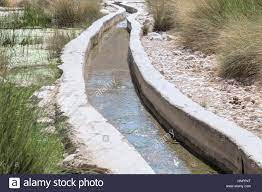
\includegraphics[width=3cm, height=2.75cm]{./figures/waterOld}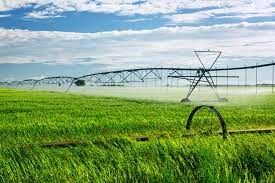
\includegraphics[width=3cm, height=2.75cm]{./figures/waterNew}
 
\end{center}
 
\end{frame}


\begin{frame}
{References}
\begin{footnotesize}
\begin{thebibliography}{1}
\bibitem[]{}{\sc OECD},
(co-author(s) if any) (year), (Title), https://data.oecd.org/canada.htm. 
\end{thebibliography}
\end{footnotesize}
\vspace{0.5cm}

\begin{center}
\footnotesize {\textbf{smoragas@sfu.ca}}, \\
\footnotesize {\textbf{sites.google.com/view/sebanthalas}}
\end{center}

\end{frame}
\end{document}
